%----------------------------------------------------------------------------------------
%	PROJECT INFORMATION
%----------------------------------------------------------------------------------------
\newcommand{\ApplicationManager}{Anakin Skywalker}
\newcommand{\ApplicationManagerDepartment}{SHS DI D\&A CEC ITH EH-PLM}
\newcommand{\ApplicationManagerContact}{\href{mailto://anakin.skywalker@siemens-healthineers.com}{anakin.skywalker\footnotemark[1]}}

\newcommand{\BusinessOwnerName}{Padme Amidala}
\newcommand{\BusinessOwnerDepartment}{SHS DI D\&A CEC EPE}
\newcommand{\BusinessOwnerContact}{\href{mailto://padme.amidala@siemens-healthineers.com}{padme.amidala\footnotemark[1]}}

\newcommand{\BusinessRepresentativeName}{Luke Skywalker}
\newcommand{\BusinessRepresentativeDepartment}{SHS DI D\&A CEC ITH EH-PLM}
\newcommand{\BusinessRepresentativeContact}{\href{mailto://luke.skywalker@siemens-healthineers.com}{luke.skywalker\footnotemark[1]}}

\newcommand{\TechnicalContactsNumber}{2}
\newcommand{\TechnicalContacts}{
	Obi Wan Kenobi &  SHS TE DC SVK D\&A DIG PTM & \href{mailto://obi-wan.kenobi@siemens-healthineers.com}{obi-wan.kenobi\footnotemark[1]} \\
	& Baby Yoda  & SHS DI D\&A CEC ITH EH-R\&D & \href{mailto://baby.yoda@siemens-healthineers.com}{baby.yoda\footnotemark[1]} \\
}

% Not needed for Scope document
% Required for Report document
\newcommand{\PentestLeadName}{Lukas Nad}
\newcommand{\PentestLeadDepartment}{SHS TE DC CYS CSA P\&PA}
\newcommand{\PentestLeadContact}{\href{mailto://lukas.nad@siemens-healthineers.com}{lukas.nad\footnotemark[1]}}



\newcommand{\PentestParticipantsNumber}{3} % Number of participants in "Penetration Testing Team"


%----------------------------------------------------------------------------------------
%	TARGET INFORMATION
%----------------------------------------------------------------------------------------
\newcommand{\TargetInfoName}{\ReportProjectName} %% Asset Name
\newcommand{\TargetInfoType}{\AssetType} %% Asset Type
\newcommand{\TargetInfoEnvironment}{Testing Environment}
\newcommand{\TargetInfoInternetFacing}{Yes} %% Asset Internet Facing
\newcommand{\TargetInfoSNXConnectivity}{No} %% SNX Connectivity
\newcommand{\TargetInfoHostingLocation}{Special Network} %% Hosting Location
\newcommand{\TargetInfoHostingProvider}{N/A} %% Hosting Provider
\newcommand{\TargetInfoLifecyclePhase}{Pre-Production}
\newcommand{\TargetInfoCriticality}{N/A}
\newcommand{\TargetInfoAssetID}{N/A}
\newcommand{\TargetInfoSHARPUUID}{N/A} %% SHARP UUID
\newcommand{\TargetInfoDescription}{Lorem ipsum dolor sit amet, consectetur adipiscing elit. Sed ultricies pharetra pretium. Cras varius purus eu cursus vehicula. Sed in molestie arcu, id placerat velit. Praesent sagittis purus in neque convallis, a faucibus odio egestas. Nam ultrices, metus et mattis facilisis, felis lectus tempor velit, a interdum nisl libero nec dui. Mauris interdum scelerisque semper. Cras mattis id lacus a ullamcorper. Curabitur fermentum vehicula leo, vel convallis turpis luctus nec. In mollis vitae diam in ornare. Donec molestie augue nisl, malesuada maximus urna gravida quis. Curabitur ac ante turpis. Nulla facilisi. Aenean eleifend ipsum at velit lobortis, in hendrerit arcu dapibus. Proin ut lacus sed tellus maximus euismod. Suspendisse elementum mauris tellus, eget imperdiet leo dictum nec. Fusce tortor mauris, iaculis non tristique ut, condimentum a odio.}

%----------------------------------------------------------------------------------------
%	AGREED TIMEFRAME
%----------------------------------------------------------------------------------------
\newcommand{\TimeframeTotal}{10 working days} 
\newcommand{\TimeframeStart}{2023-05-29} 
\newcommand{\TimeframeEnd}{2023-06-09} 
\newcommand{\TimeframeReportDue}{2023-06-12} 
\newcommand{\TimeframeComment}{-}

%----------------------------------------------------------------------------------------
%	FINDINGS COUNT AND OVERALL THREAT EXPOSURE
%----------------------------------------------------------------------------------------
% Not needed for Scope document
% Required for Report document

\newcommand{\OverallThreatExposureImage}{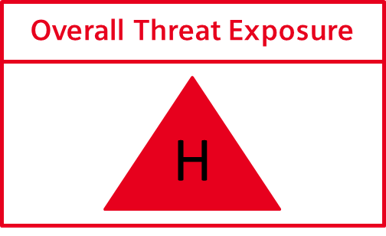
\includegraphics{Images/HighThreat.png}} 
% 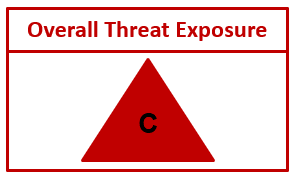
\includegraphics{Images/CriticalThreat.png}, 
% 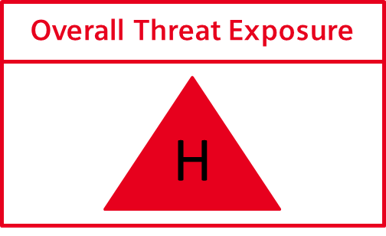
\includegraphics{Images/HighThreat.png}, 
% \includegraphics{Images/MediumThreat.png}, 
% 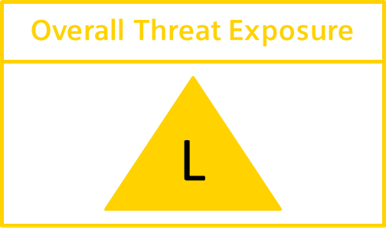
\includegraphics{Images/LowThreat.png}

\newcommand{\FindingsCountCritical}{0}
\newcommand{\FindingsCountHigh}{1}
\newcommand{\FindingsCountMedium}{2}
\newcommand{\FindingsCountLow}{2}
\newcommand{\FindingsCountInfo}{2}
\newcommand{\FindingsCountTotal}{7}